\chapter{Testing}
Throughout the development of Job Crop, testing was done to regularly iterate and change this web application to meet the stakeholder's needs. The testing methods used through the development stage are described in this chapter.

In the early stages of Implementation, Goldsmiths HR was contacted to make sure what it is that employers would want from a web application such as this and to gain more understanding of the perspective of an employer. But, Goldsmiths HR Team didn't reply to the request and as a result the Employers design was not completely tested. To test the employers design and needs, a person who imitated an employer was used. More details about this test is given in the User Testing section.

Other than User testing, Functional Testing, Compatibility Testing, Security Testing and Performance Testing were done to confirm that the web app works as expected. Unit tests were also written for each file and run to check if everything worked as expected. Compatibility Testing was also done to ensure the web app behaved the same way in different browsers and devices.

Throughout the development and testing phase, the users and stakeholders generally liked the idea of this project as they had also faced many difficulties using a traditional job search engine. This helped me gain valuable feedback and helped build the web app.

\section{Functional Testing}
Functional Testing was done on this web app to ensure the proper working of the web application's functionalities. Functional Testing is a type of software testing that validates the software system against the functional requirements/specifications. Functional tests test each function of the software application by providing appropriate input and verifying the output against the Functional requirements. \parencite{Reference36}

Functional testing mainly involves black box testing, and it is not concerned with the source code of the application. This testing checks the User Interface, APIs, Database, Security, Client/Server communication and other functionality of the Application Under Test. The testing can be done either manually or using automation. 

\subsection{Functional Testing Scenarios}

\begin{itemize}
    \item Test all the mandatory fields should be validated.

    \textbf{Result: Passed}

    \item Test the system should not display the error message for optional fields.

    \textbf{Result: Passed}

    \item Test that an error message should display for errors.

    \textbf{Result: Passed}

    Error messages display when a user writes the wrong email/password.

    \item Test the JavaScript is properly working in different browsers

    \textbf{Result: Passed}

    \item Test to see what happens if a user deletes cookies while on the site.

    \textbf{Result: Passed}
    
    When cookies are deleted, the user's login information is deleted, redirecting the user to the home page.

    \item Test after login, the user is able to see their job matches

    \textbf{Result: Passed}
\end{itemize}


\section{Compatibility Testing}
To make sure the web app was compatible with the necessary systems it should work, Compatibility testing was important. Due to time constraints, the "/matches" route of the web app is not completely compatible with any device with a width of 9 inches or lesser (595px or lesser). Making this web app usable on mobile phones is considered a vital part of its future work.

\subsection{Compatibility Testing scenarios}
\begin{itemize}
    \item Test the website in different browsers (IE, Firefox, Chrome, Safari, and Opera) and ensure the website is displaying properly.

    \textbf{Result: Passed}
    
    The website was tested on different browsers like Chrome, Firefox, Safari and Brave, and they all were fully compatible with all of them. All the web pages were displaying as expected, and the performance wasn’t compromised. The images and fonts were also displayed as expected.

    \item Test the JavaScript code is usable in different browsers

    \textbf{Result: Passed}

    The JavaScript code is usable in all browsers mentioned above.

    \item Test if the website is usable with JavaScript disabled

    \textbf{Result: Failed}

    As this web app is completely built on React, JavaScript needs to be enabled for this web app to run.

    \item Check if the website works with cookies disabled

    \textbf{Result: Passed}
\end{itemize}

\newpage
\section{Security Testing}
To ensure that this web app is secure and to identify the threats in the system and measure its potential vulnerabilities, security testing is done on this web application. 

\subsection{Security Testing Scenarios}
\begin{itemize}
    \item Verify the web page, which contains important data like passwords, credit card numbers, secret answers for security questions etc., should be submitted via HTTPS (SSL).

    \textbf{Result: Failed}

    As this web app is built completely on the local host, sensitive data is not submitted via HTTPS or SSL but this can be fixed once this website is hosted.

    \item Verify that important information like passwords, credit card numbers etc,  should display in an encrypted format.

    \textbf{Result: Passed}

    Passwords are shown in an encrypted format which can't be seen. Refer Figure \ref{fig:login-page-redacted}

    \item Verify if the password is changed; the user should not be able to log in with the old password.

    \textbf{Result: Passed}
    
    If a user's password is changed in the database, the user cannot log in with the old password. This is made sure by Firebase's real-time cloud updates, which checks the database each time the request is sent.


    \item Access a page which does not exist and ensure the user is redirected to the homepage

    \textbf{Result: Passed }
    
    If a user attempts to go to a route which does not exist, they are redirected to the homepage. This is done through the following code:

    \begin{lstlisting}
    <Route path="*" element={<Home />} />
    \end{lstlisting}

    \item Verify the user account gets locked out if the user enters the wrong password several times.

    \textbf{Result: Failed}

    The result shows that no user account locked-out function has been implemented. Which is vulnerable to dictionary attacks with common usernames and passwords, which is not secure. A functionality to lock out a user upon multiple wrong password attempts must be created.

    \item Verify if any SQL injection attacks can be taken place in the input fields.

    \textbf{Result: Passed}

    Firebase does not build a SQL command to execute a query, meaning SQL Injection can't be done on this web app. 
\end{itemize}

\begin{figure}
    \centering
    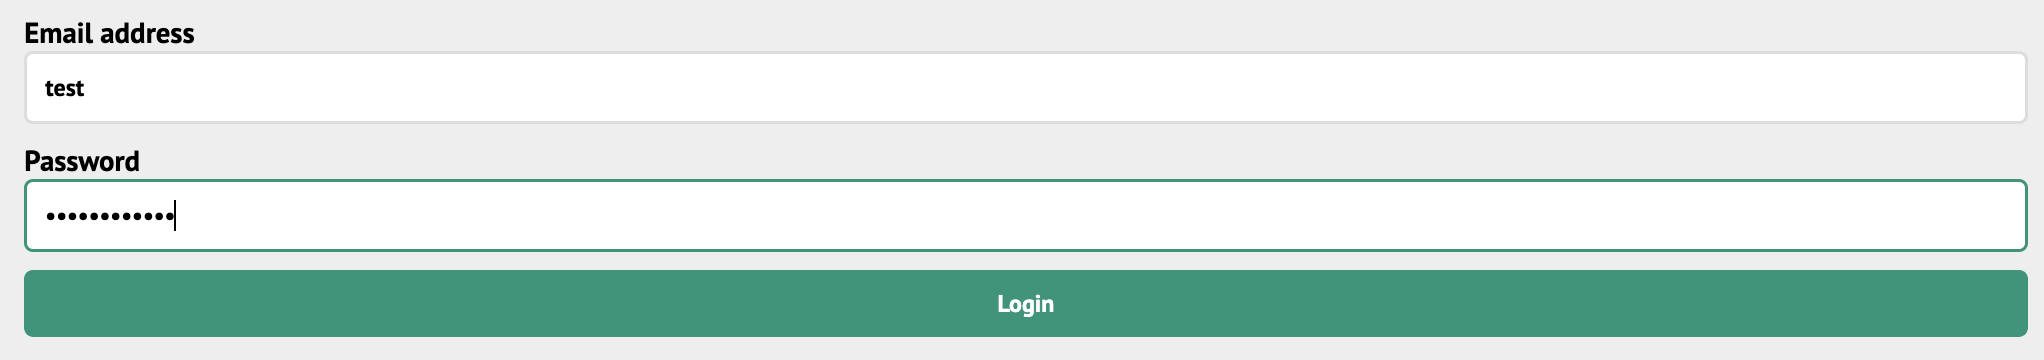
\includegraphics[width=140mm]{Figures/login-page-redacted.png}
    \caption{The password input can be seen as redacted.}
    \label{fig:login-page-redacted}
\end{figure}

\section{Performance Testing}
This web application was tested on different devices like MacBooks, PCs, and a couple of Android devices, as well as Google Chromebooks with different browsers like Firefox, Chrome, Safari, and Brave and the performance of our website, was never compromised by any of the devices or browsers used.

\section{Database Testing}
Database testing is a type of software testing that checks the schema, tables, etc., of the Database. It also checks data integrity and consistency. Testing the database for any web application is very important.

\subsection{Database Testing Scenarios}
\begin{itemize}
    \item Verify the database name: The database name should match the specifications.

    \textbf{Result: Passed}

    Each database is named according to its specifications

    \item Verify the Tables, columns, column types and defaults: All things should match the specifications.

    \textbf{Result: Passed}

    All the tables, column names, and types match their specifications.

    \item Verify the Primary and foreign keys of each table.

    \textbf{Result: Passed}

    Each table's primary and foreign keys are the same as in the ERD in Figure \ref{fig: Entity Relationship Diagram}.

    \item Verify if the data in the database is encrypted.

    \textbf{Result: Failed}

    While this should be done in the future, during the development stage, it didn't feel like this would be needed and as a result the data is not encrypted in the database.

    \item Verify the data validity by inserting the invalid data into the database.

    \textbf{Result: Passed}

    If invalid data is passed into the database, it throws an error.
\end{itemize}


\section{Unit Testing}

To make sure all code meets quality standards before it is deployed, Unit Tests are created using Jest. Jest is a JavaScript Testing Framework which helps in testing and works particularly well with React \parencite{Reference34}. Jest tests are written for each JavaScript component and can be seen throughout the codebase. Component tests are named according to the industry standard with \textit{X.test.js} where X is the component's name. Below is an example of a test written in Jest:

\begin{lstlisting}
it('should render a button with text "Try it now!"', () => {
    render(<Features />);
    const button = screen.getByText('Try it now!');
    expect(button).toBeInTheDocument();
    expect(button.tagName).toBe('BUTTON');
});
\end{lstlisting}
At first, the test renders the component Features and gets the Button with its unique text: "Try it now!". Here, expect is the expectation of what the code should do. The const button gets the Button by its text and then expects the Button to be in the document and have the tagName Button. There are only two expect statements in this code, but more can be added to improve code coverage with time like 
\begin{lstlisting}
expect(button.className).toBe('login-button');
\end{lstlisting}

The tests were done locally throughout the development period, and more dependencies were added to the package.json file. The dependencies added for testing are shown below
\begin{lstlisting}
"devDependencies": {
    "@testing-library/jest-dom": "^5.16.5",
    "@testing-library/react": "12.1.2",
    "jest": "24.9.0",
    "react-test-renderer": "^18.2.0"
}
\end{lstlisting} 

ESLint was also used throughout the development process. It analyses code to find problems, such as unused variables and helps make the whole codebase have the same syntax as it automatically finds syntax errors and fixes them. 

\section{User Testing}
\subsection{Employer Design Testing}
A tester was used to identify what potential roles an employer would want to use in an application such as this. It is important to note that this tester had no previous HR Experience. This tester was used to gain an understanding of what employers would want to do with this web application. After providing with an overall description of what this web application was, a conversation was had to better understand employer's needs from this web application. Below is a rough conversation I had with the tester:

Me: What do you think a potential employer would want to do in an application such as this?

Tester: I think I would want a platform that is easy to navigate and use to post job openings quickly and efficiently.

Me: Imagine you're currently posting a job on this application. What are the things you would like to see while doing this task?

Tester: I would like the platform to first let me navigate easily to the page where I can post the job. When posting the job, I would like to be able to post it successfully. I would also like the options to customise the job post.

Me: Can you provide more information about what you would like to customise?

Tester: Sure, I would like to be able to customise my job postings with information that I want. This includes company description, job position, values, requirements, minimum qualifications, etc. I would like to be able to showcase the company brand and culture through the job posting.

Me: Can you please tell me what Analytics you would like to see in a job application such as this?

Tester: Off the top of my head, I'd like to know how many views and applications each posting received.

Me: Great, thanks. Is there anything else you would like to add before finishing up?

Tester: Well, not really. Just Good luck.

Me: Thank you and Thanks for taking the time to speak with me.

This conversation showed that most of the application's employer's requirements were all acknowledged. Employers will be able to fully customise their job postings on the web application and will be able to update/edit/delete applications. They will also be able to see the analytics and data behind each job when the development process of this web application is complete.

\subsection{Applicant Design Testing}
User experience and design are pretty important to any application, so during the development stage, the web app was tested with users. The designs at the start of the project were shown to a group of 10 people, and their feedback was recorded. The designs shown to them were Figures \ref{fig: Home Screen}, \ref{fig: Job Posting} and \ref{fig: Login Page}. The responses are given in figures \ref{fig:home-screen-responses}, \ref{fig:login-page-responses} and \ref{fig:job-posting-responses}

\begin{figure}
    \centering
    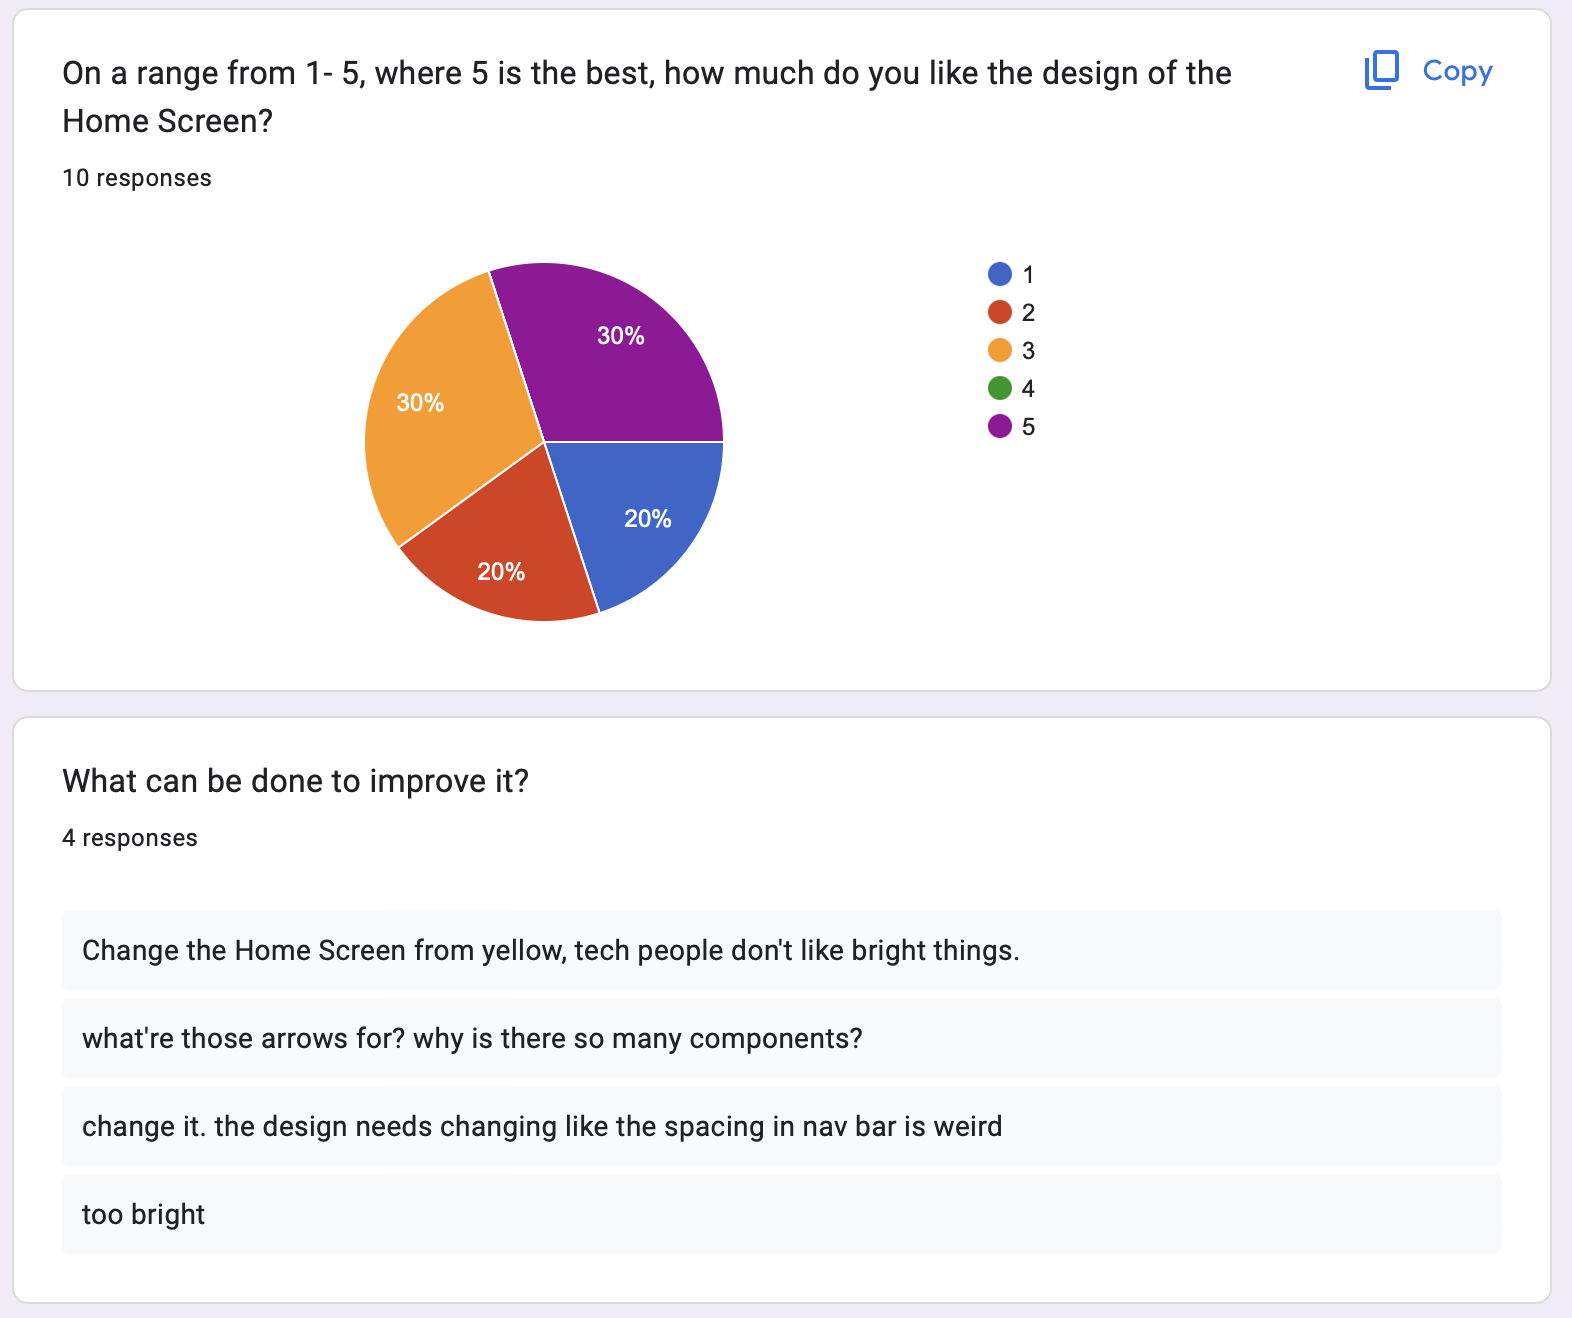
\includegraphics[width=140mm]{Figures/home-screen.png}
    \caption{Responses to the Home Screen Page}
    \label{fig:home-screen-responses}
\end{figure}
\begin{figure}
    \centering
    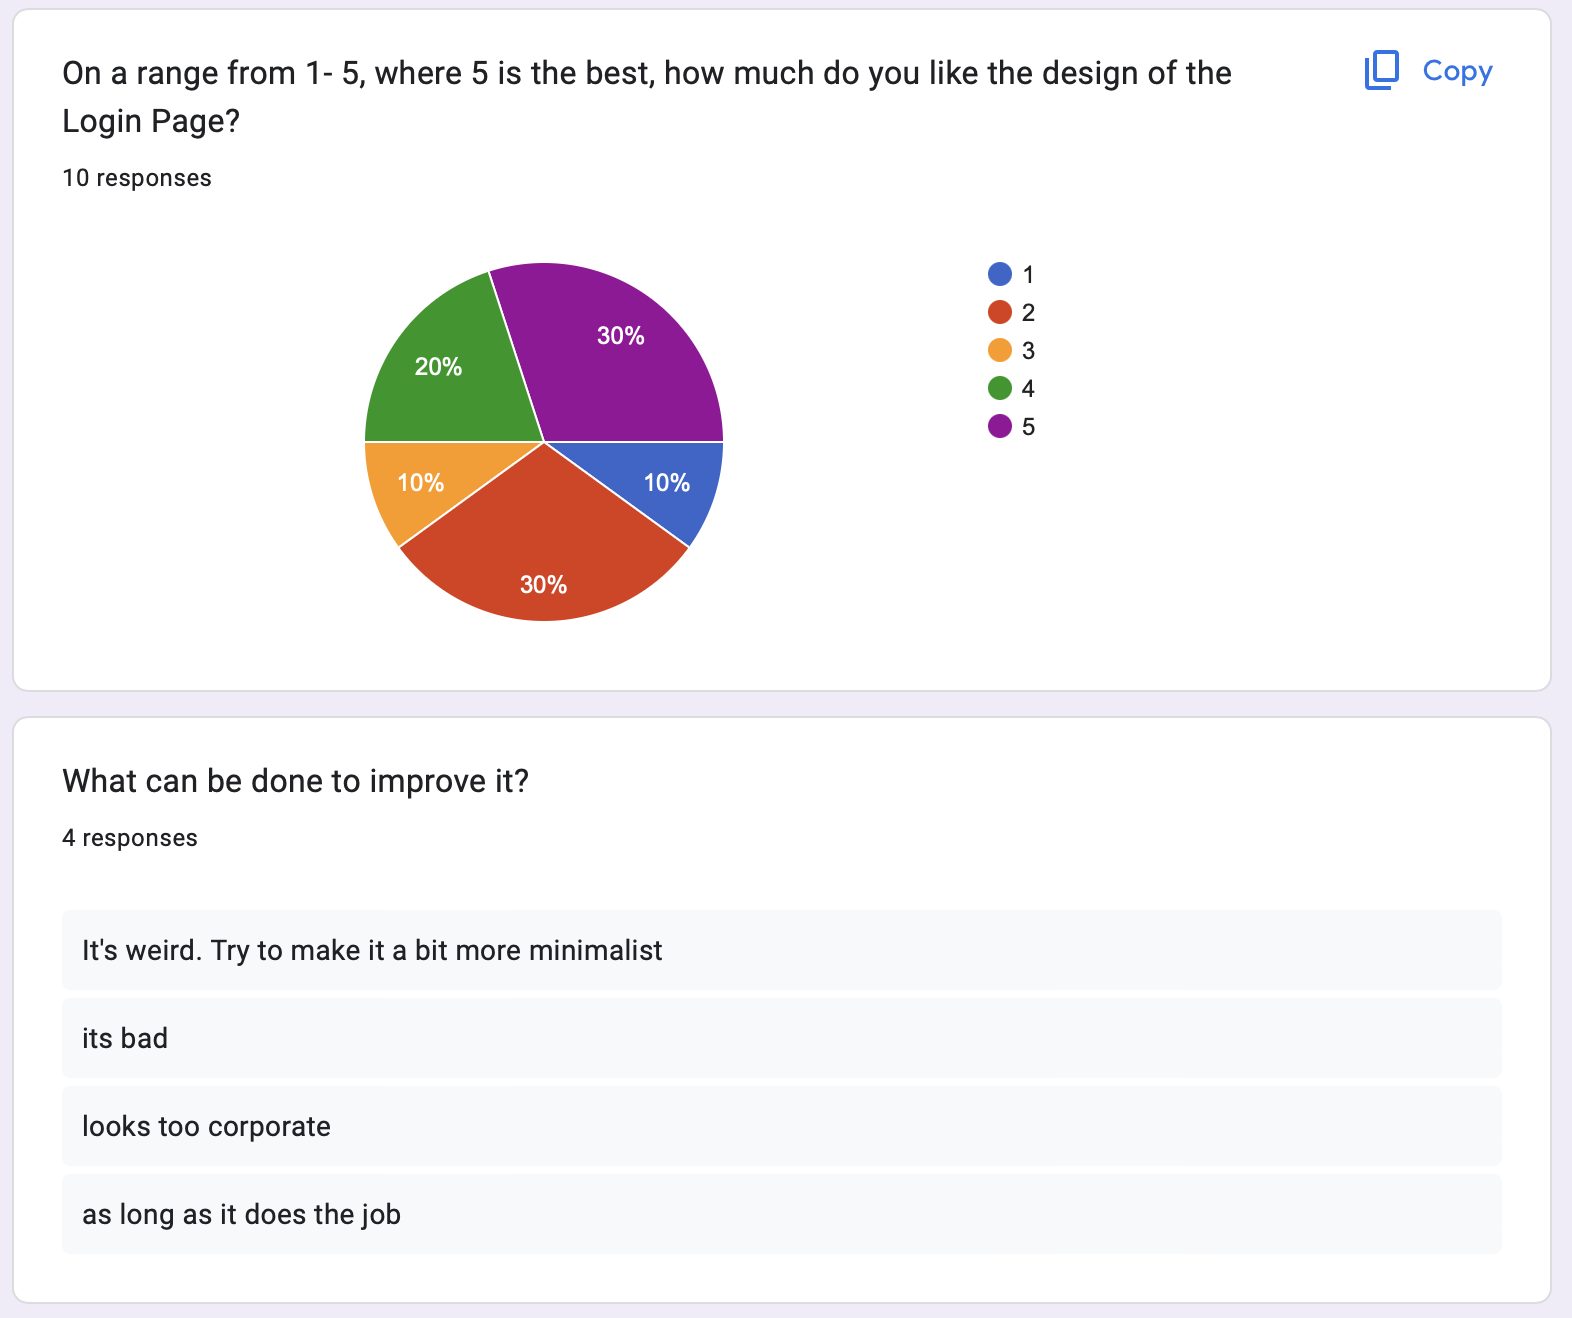
\includegraphics[width=140mm]{Figures/login-page.png}
    \caption{Responses to the Login Page}
    \label{fig:login-page-responses}
\end{figure}
\begin{figure}
    \centering
    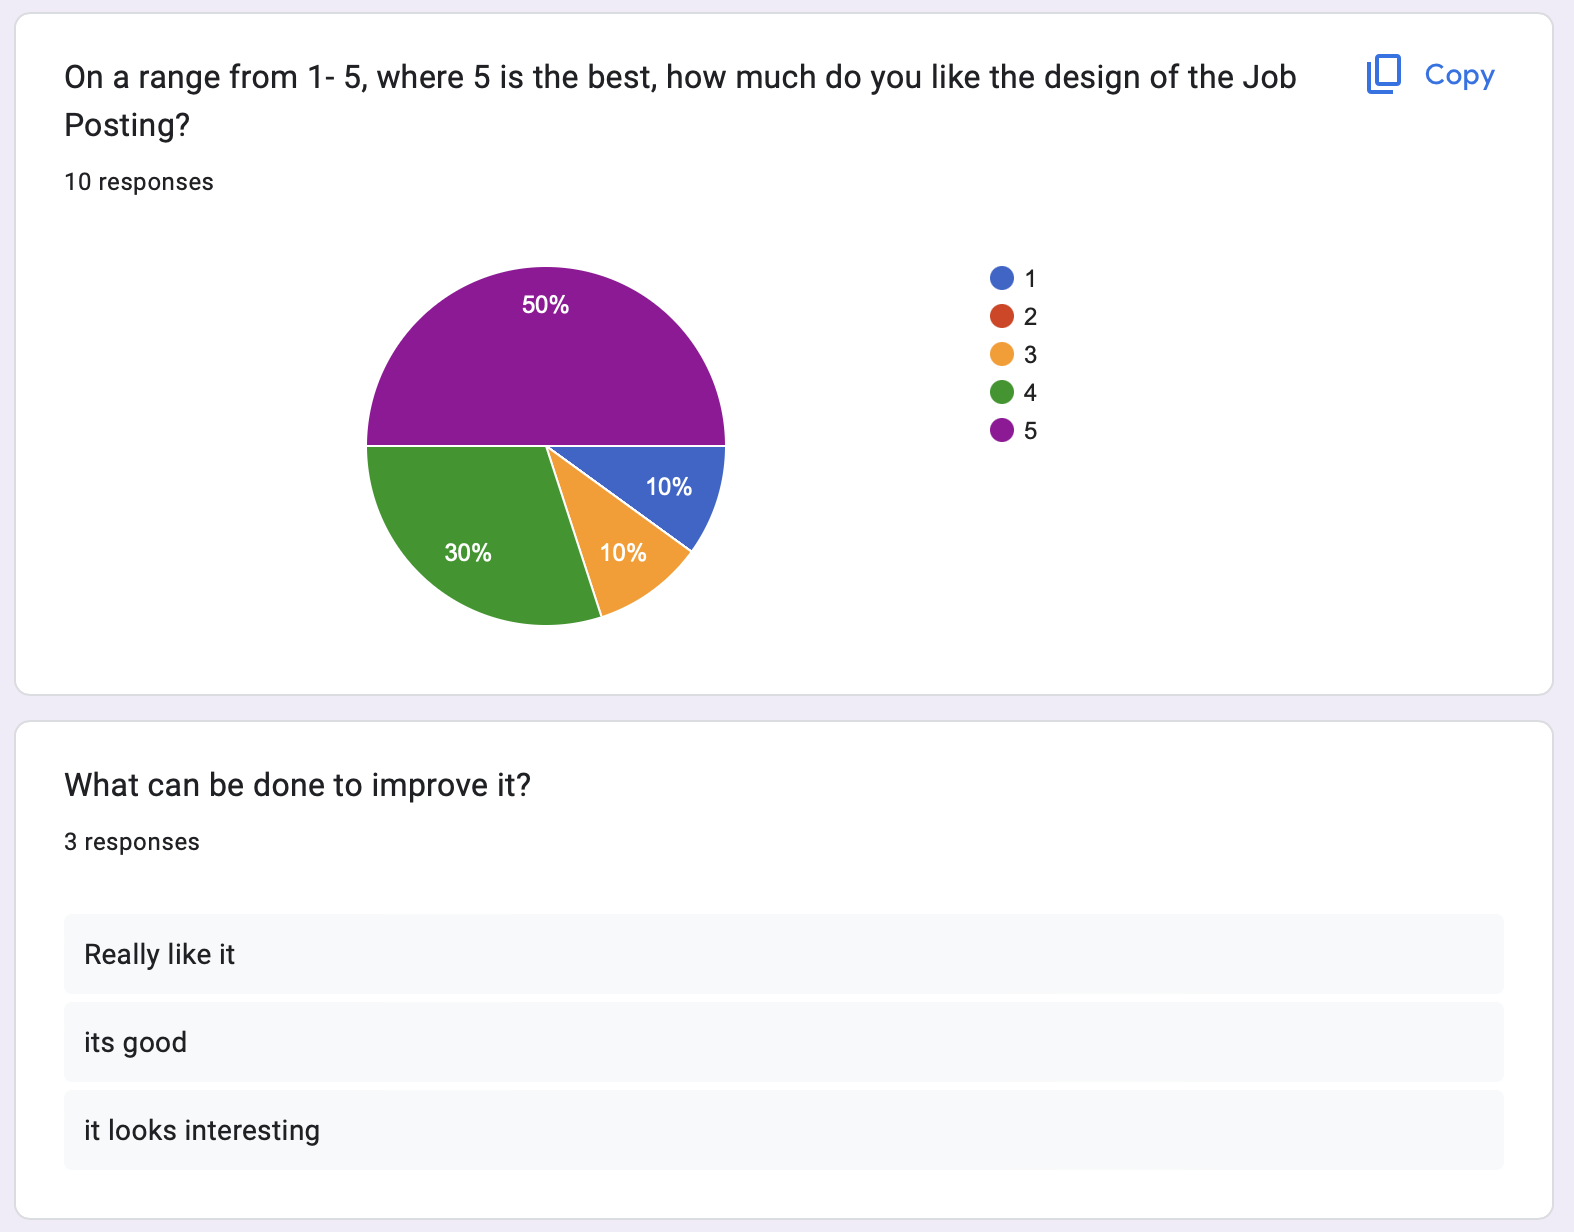
\includegraphics[width=140mm]{Figures/job-posting.png}
    \caption{Responses to the Job Posting Page}
    \label{fig:job-posting-responses}
\end{figure}

Designs were changed in the development process according to these responses. As can be seen, only 30\% of people rated the home screen as five and 50\% rated it as 1 or 2. This meant the home screen needed changing. As a result, the improvements that were conveyed by the testers were taken into account. The home screen was changed from yellow to dark, the arrows were removed, and the number of elements on the screen was reduced.

The login Page was also changed to make it more "minimalist". The background image was removed, and only the required components were kept.

Testers seemed satisfied with the Job Postings page, so it was not changed significantly, but the names of buttons were added to ensure users knew what Button they clicked.

\subsection{Usability Testing}
A total of seven testers were asked to complete the Usability Testing. The number of testers was low as this web application was built entirely locally, and testers needed the machine in which this application was being made to test the application. This, while an inconvenience, worked really well as I was able to see where the testers were trying to go for each prompt asked of them and were also able to time them. This testing was done in one day, and as participants had to wait to test the app on my local computerg, the number of questions in this testing was kept as low as possible. 

A time limit of 10 seconds was kept for each task to be completed. This time limit was not shared with the testers to keep them at ease.

The following guideline was given to the testers before starting the test:

\textit{"The question will ask you to perform a task. These tasks are time but please perform these them at ease. These tasks are performed under timed conditions only because we are testing how long a task takes. This session is designed to make this web application more intuitive and user-friendly. If you are unable to perform the said task, do not worry. We'd love to hear your feedback."}

The tasks the testers had to perform were:

\textbf{Task 1:} Please navigate to these web pages on the application: About Page, For Employers Page and Sign In Page.

All testers were able to access each of these web pages within the time limit.

\textbf{Task 2:} Can you please describe the loading times of the web pages?

All testers were happy with the loading times of the application. Their responses are shown in Figure \ref{fig:usability-responses}

\begin{figure}
    \centering
    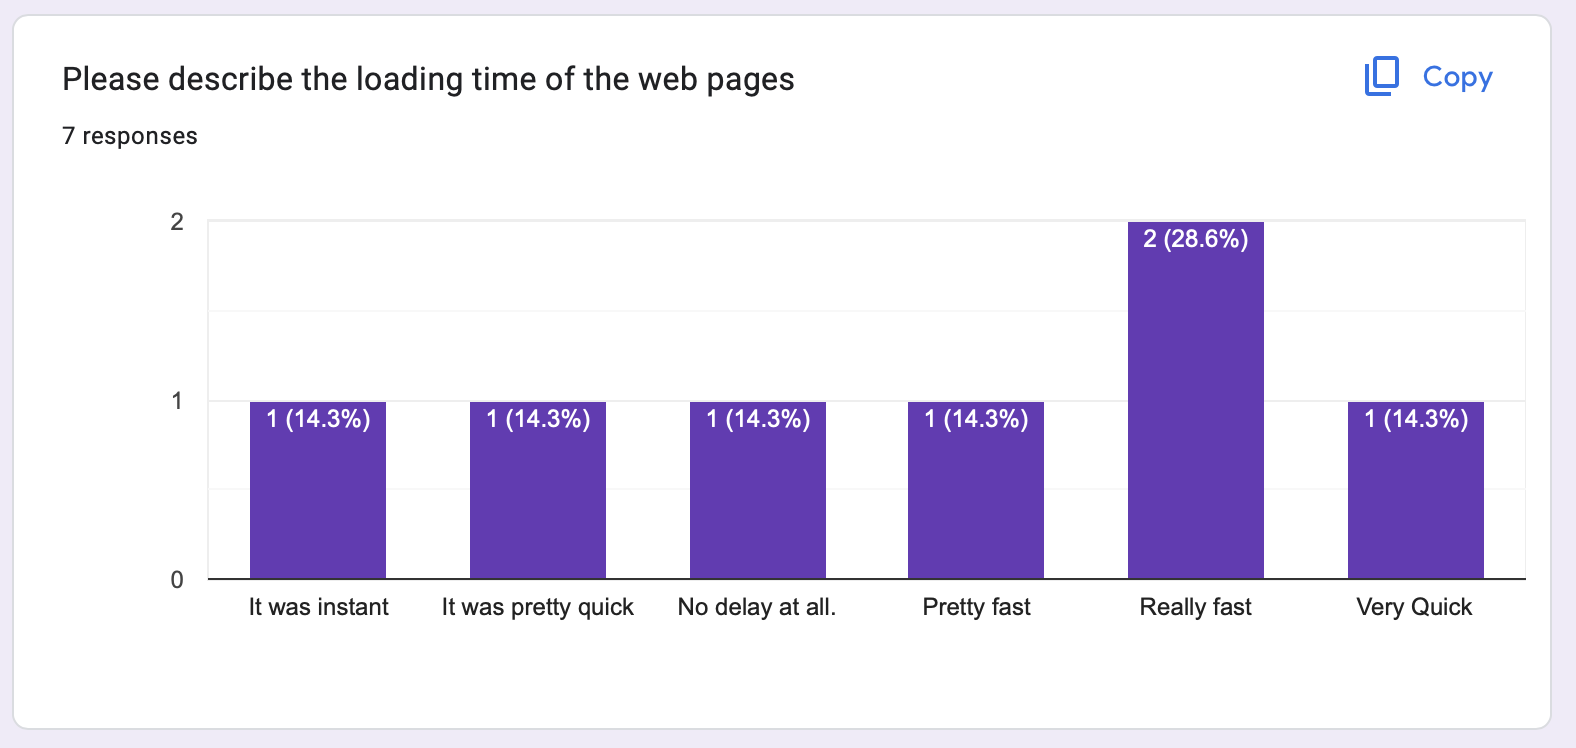
\includegraphics[width=140mm]{Figures/usability-responses}
    \caption{Responses from testers for Task 2}
    \label{fig:usability-responses}
\end{figure}

\textbf{Task 3:} Are the webpage's names self-explanatory? Would you change the name of any link names?

All testers were happy with the web page names and thought it was self-explanatory, except for one who mistook the Employers Page to be the page they had to click to get matches from employers. As a result, the name of the link was changed to "For Employers" page.

Their responses are shown in Figure \ref{fig:self-explanatory-pages}.

\begin{figure}
    \centering
    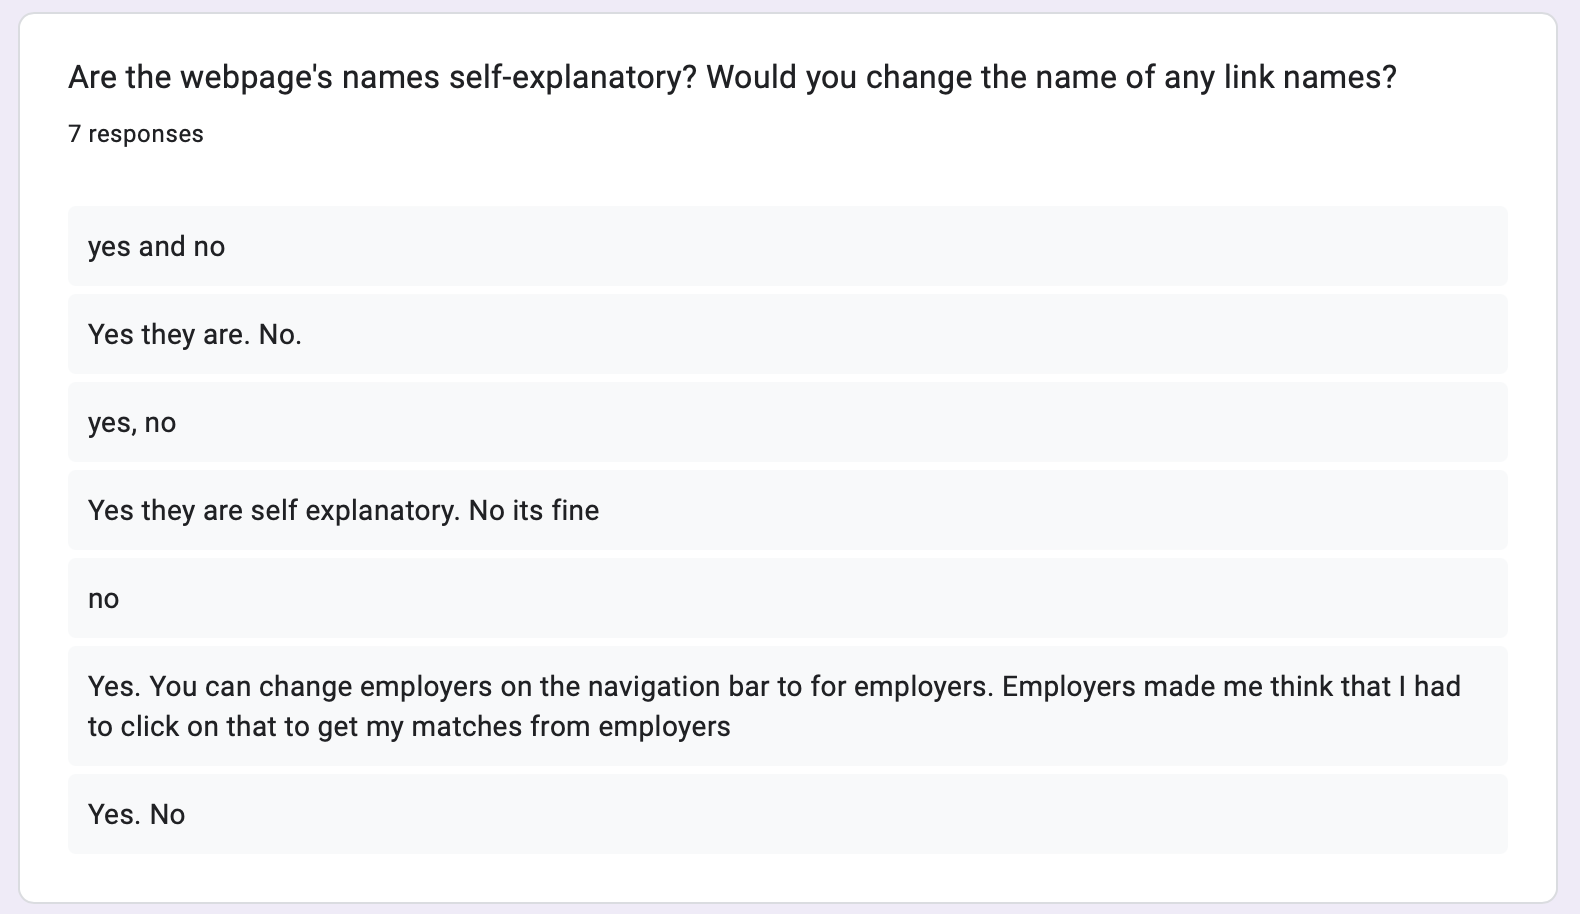
\includegraphics[width=140mm]{Figures/self-explanatory-pages.png}
    \caption{Responses from Testers for Task 3}
    \label{fig:self-explanatory-pages}
\end{figure}

\textbf{Task 4:} Please login with the username and password jbond007@gold.ac.uk. Can you do it and see the potential match?

Three testers took about twenty seconds to complete this task, the other two took forty seconds, and the last two took about a minute to complete this task. While the time taken to complete this task varied with testers, the three testers who completed it in twenty seconds got the password right the first time, while the other two took three attempts to get it right. The last two couldn't understand what the password was on the first attempt reading the question. This was due to the wording of the question.

\textbf{Task 5:} Would you like to give any additional feedback?

As there were no error messages shown on the login page at the time of this testing, many testers complained about adding an error message there. After this testing, error messages were added when a user gave the wrong email/password.

Their responses are shown in Figure \ref{fig:Feedback-responses}.

\begin{figure}
    \centering
    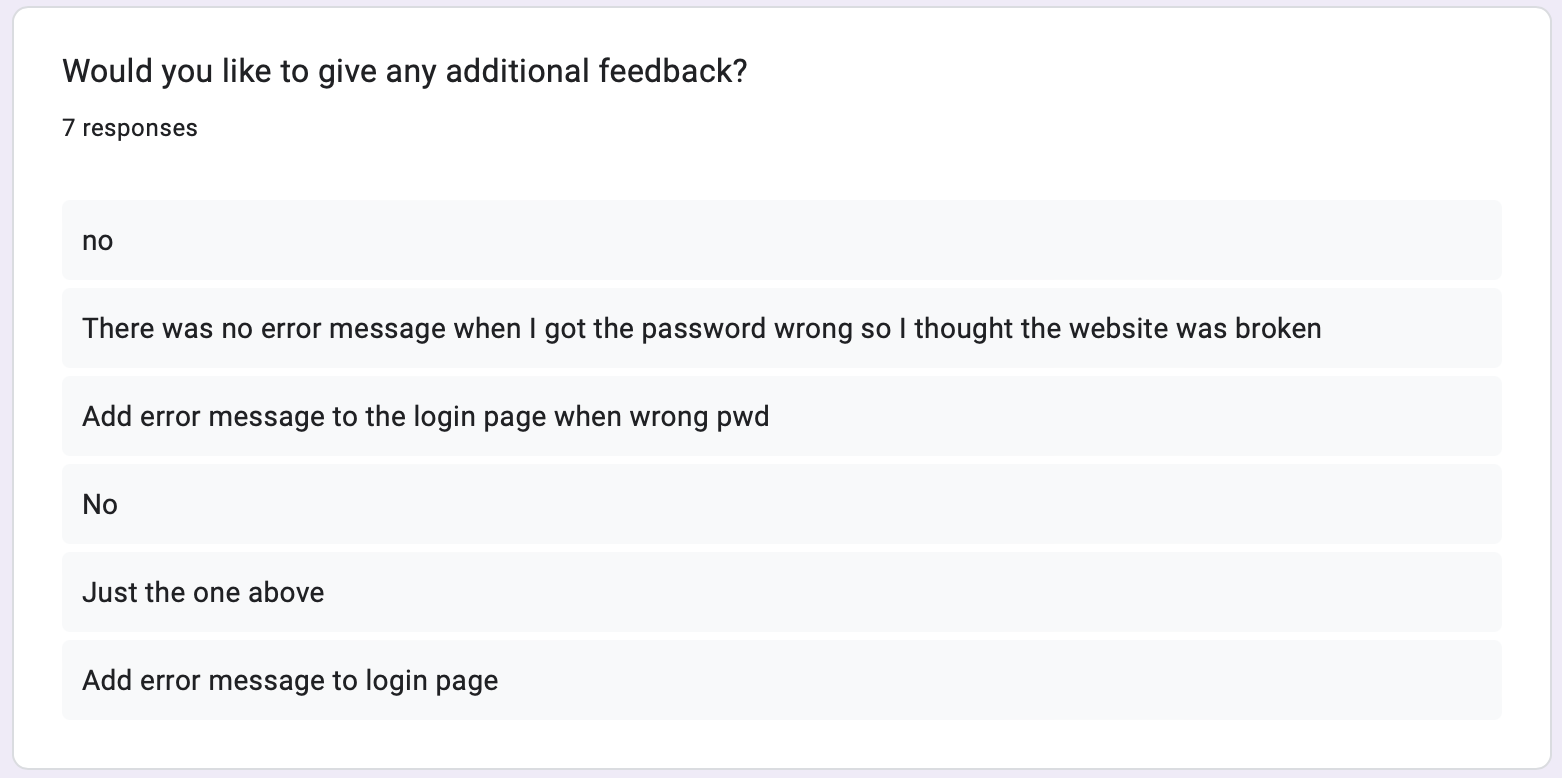
\includegraphics[width=140mm]{Figures/Feedback-responses.png}
    \caption{Responses from Testers for Task 5}
    \label{fig:Feedback-responses}
\end{figure}

\subsubsection{Usability Testing Conclusion}
Usability testing worked really well for the application as most testers were happy with the application other than a few couple of things which were fixed upon feedback. Every tester was able to complete all tasks in the web application, and the additional feedback shows that testers were overall happy with the application except for a few places. 

\section{Testing conclusion}
After conducting such comprehensive testing on the web application, it can be concluded that the app meets majority of its objectives and requirements. Some test scenarios did fail which have raised more issues that need to be resolved. Some more areas in need of development work are also identified such as the need to security measures to encrypt data of users. Conducting these tests was extremely useful and many improvements are needed in the application before its implementation is completed. 

There is more user testing needed for the currently built pages but as these were built close to the deadline, the testing couldn't be completed in time. That is the only testing left to do in this web application and will be done in due time.

\section{Ethical Compliancy for Testing} 
It should also be noted that testers in all these studies wished to remain anonymous and all of them were aged 18 or above.